\documentclass[12pt, a4paper,  BCOR=8.25mm, DIV=15]{scrartcl}\usepackage[]{graphicx}\usepackage[]{color}
%% maxwidth is the original width if it is less than linewidth
%% otherwise use linewidth (to make sure the graphics do not exceed the margin)
\makeatletter
\def\maxwidth{ %
  \ifdim\Gin@nat@width>\linewidth
    \linewidth
  \else
    \Gin@nat@width
  \fi
}
\makeatother

\definecolor{fgcolor}{rgb}{0.345, 0.345, 0.345}
\newcommand{\hlnum}[1]{\textcolor[rgb]{0.686,0.059,0.569}{#1}}%
\newcommand{\hlstr}[1]{\textcolor[rgb]{0.192,0.494,0.8}{#1}}%
\newcommand{\hlcom}[1]{\textcolor[rgb]{0.678,0.584,0.686}{\textit{#1}}}%
\newcommand{\hlopt}[1]{\textcolor[rgb]{0,0,0}{#1}}%
\newcommand{\hlstd}[1]{\textcolor[rgb]{0.345,0.345,0.345}{#1}}%
\newcommand{\hlkwa}[1]{\textcolor[rgb]{0.161,0.373,0.58}{\textbf{#1}}}%
\newcommand{\hlkwb}[1]{\textcolor[rgb]{0.69,0.353,0.396}{#1}}%
\newcommand{\hlkwc}[1]{\textcolor[rgb]{0.333,0.667,0.333}{#1}}%
\newcommand{\hlkwd}[1]{\textcolor[rgb]{0.737,0.353,0.396}{\textbf{#1}}}%

\usepackage{framed}
\makeatletter
\newenvironment{kframe}{%
 \def\at@end@of@kframe{}%
 \ifinner\ifhmode%
  \def\at@end@of@kframe{\end{minipage}}%
  \begin{minipage}{\columnwidth}%
 \fi\fi%
 \def\FrameCommand##1{\hskip\@totalleftmargin \hskip-\fboxsep
 \colorbox{shadecolor}{##1}\hskip-\fboxsep
     % There is no \\@totalrightmargin, so:
     \hskip-\linewidth \hskip-\@totalleftmargin \hskip\columnwidth}%
 \MakeFramed {\advance\hsize-\width
   \@totalleftmargin\z@ \linewidth\hsize
   \@setminipage}}%
 {\par\unskip\endMakeFramed%
 \at@end@of@kframe}
\makeatother

\definecolor{shadecolor}{rgb}{.97, .97, .97}
\definecolor{messagecolor}{rgb}{0, 0, 0}
\definecolor{warningcolor}{rgb}{1, 0, 1}
\definecolor{errorcolor}{rgb}{1, 0, 0}
\newenvironment{knitrout}{}{} % an empty environment to be redefined in TeX

\usepackage{alltt}
\usepackage[utf8]{inputenc}
\usepackage{newfloat}
\usepackage{float}
\DeclareFloatingEnvironment[name={Supplementary Figure}]{suppfigure}

\newenvironment{itemizz}%
  {\begin{itemize}%
    \setlength{\itemsep}{2pt}%
    \setlength{\parskip}{2pt}}%
  {\end{itemize}}

\newcommand{\txtt}[1]{{\texttt{#1}}}
\IfFileExists{upquote.sty}{\usepackage{upquote}}{}
\begin{document}
%\VignetteEngine{knitr::knitr}
%\VignetteIndexEntry{Regression (Set 11)}




\title{11: Regression}
\author{John H Maindonald}
\maketitle

\vspace*{-1cm}

\begin{knitrout}
\definecolor{shadecolor}{rgb}{0.969, 0.969, 0.969}\color{fgcolor}\begin{kframe}
\begin{alltt}
\hlstd{fig11.1} \hlkwb{<-} \hlkwa{function}\hlstd{()\{}
\hlcom{## ---- plt-roller ----}
\hlkwd{plot}\hlstd{(depression} \hlopt{~} \hlstd{weight,} \hlkwc{data}\hlstd{=roller)}
\hlstd{\}}
\end{alltt}
\end{kframe}
\end{knitrout}

\begin{knitrout}
\definecolor{shadecolor}{rgb}{0.969, 0.969, 0.969}\color{fgcolor}\begin{kframe}
\begin{alltt}
\hlstd{fig11.2} \hlkwb{<-} \hlkwa{function}\hlstd{()\{}
\hlcom{## ---- pltWline ----}
\hlkwd{plot}\hlstd{(depression} \hlopt{~} \hlstd{weight,} \hlkwc{data}\hlstd{=roller)}
\hlstd{roller.lm} \hlkwb{<-} \hlkwd{lm}\hlstd{(depression} \hlopt{~} \hlstd{weight,} \hlkwc{data}\hlstd{=roller)}
\hlcom{# For a line through the origin, specify}
\hlcom{# depression ~ 0 + weight}
\hlkwd{abline}\hlstd{(roller.lm)}
\hlstd{\}}
\end{alltt}
\end{kframe}
\end{knitrout}

\begin{knitrout}
\definecolor{shadecolor}{rgb}{0.969, 0.969, 0.969}\color{fgcolor}\begin{kframe}
\begin{alltt}
\hlstd{fig11.3} \hlkwb{<-} \hlkwa{function}\hlstd{()\{}
\hlcom{## ---- fVSmTime ----}
\hlkwd{xyplot}\hlstd{(timef}\hlopt{~}\hlstd{time,} \hlkwc{data}\hlstd{=nihills,} \hlkwc{aspect}\hlstd{=}\hlnum{1}\hlstd{,}
       \hlkwc{type}\hlstd{=}\hlkwd{c}\hlstd{(}\hlstr{"p"}\hlstd{,}\hlstr{"r"}\hlstd{))}
\hlstd{\}}
\end{alltt}
\end{kframe}
\end{knitrout}


\begin{knitrout}
\definecolor{shadecolor}{rgb}{0.969, 0.969, 0.969}\color{fgcolor}\begin{kframe}
\begin{alltt}
\hlstd{fig11.4} \hlkwb{<-} \hlkwa{function}\hlstd{()\{}
\hlcom{## ---- mfdensity ----}
\hlcom{## Simplified code}
\hlkwd{densityplot}\hlstd{(}\hlopt{~} \hlstd{time}\hlopt{+}\hlstd{timef,} \hlkwc{data}\hlstd{=nihills,}
            \hlkwc{ylab}\hlstd{=}\hlstr{"Time (h)"}\hlstd{,} \hlkwc{auto.key}\hlstd{=}\hlnum{TRUE}\hlstd{)}
\hlstd{\}}
\end{alltt}
\end{kframe}
\end{knitrout}

\begin{knitrout}
\definecolor{shadecolor}{rgb}{0.969, 0.969, 0.969}\color{fgcolor}\begin{kframe}
\begin{alltt}
\hlstd{fig11.5} \hlkwb{<-} \hlkwa{function}\hlstd{()\{}
\hlkwd{print}\hlstd{(}\hlstr{"Run the separate functions fig11.5A() and fig11.5B()"}\hlstd{)}
\hlstd{\}}
\hlstd{fig11.5A} \hlkwb{<-} \hlkwa{function}\hlstd{()\{}
\hlcom{## ---- rec-logmf ----}
\hlkwd{xyplot}\hlstd{(timef}\hlopt{~}\hlstd{time,} \hlkwc{data}\hlstd{=nihills,}
       \hlkwc{scales}\hlstd{=}\hlkwd{list}\hlstd{(}\hlkwc{log}\hlstd{=}\hlnum{10}\hlstd{),}
       \hlkwc{aspect}\hlstd{=}\hlnum{1}\hlstd{,} \hlkwc{type}\hlstd{=}\hlkwd{c}\hlstd{(}\hlstr{"p"}\hlstd{,}\hlstr{"r"}\hlstd{))}
\hlstd{\}}
\hlstd{fig11.5B} \hlkwb{<-} \hlkwa{function}\hlstd{()\{}
\hlcom{## ---- skewtime-log ----}
\hlkwd{densityplot}\hlstd{(}\hlopt{~} \hlkwd{log}\hlstd{(time)}\hlopt{+}\hlkwd{log}\hlstd{(timef),} \hlkwc{data}\hlstd{=nihills,}
           \hlkwc{ylab}\hlstd{=}\hlstr{"Time (h)"}\hlstd{,} \hlkwc{auto.key}\hlstd{=}\hlnum{TRUE}\hlstd{)}
\hlstd{\}}
\end{alltt}
\end{kframe}
\end{knitrout}

\begin{knitrout}
\definecolor{shadecolor}{rgb}{0.969, 0.969, 0.969}\color{fgcolor}\begin{kframe}
\begin{alltt}
\hlstd{fig11.6} \hlkwb{<-} \hlkwa{function}\hlstd{()\{}
\hlkwd{print}\hlstd{(}\hlstr{"Run the separate functions fig11.6A() and fig11.6B()"}\hlstd{)}
\hlstd{\}}
\hlstd{fig11.6A} \hlkwb{<-} \hlkwa{function}\hlstd{()\{}
\hlcom{## Panel A}
\hlkwd{plot}\hlstd{(}\hlkwd{resid}\hlstd{(mftime.lm)}\hlopt{~}\hlstd{time,} \hlkwc{data}\hlstd{=nihills)}
\hlkwd{mtext}\hlstd{(}\hlkwc{side}\hlstd{=}\hlnum{3}\hlstd{,} \hlkwc{line}\hlstd{=}\hlnum{0.5}\hlstd{,} \hlstr{"A: Residuals, unlogged data"}\hlstd{)}
\hlstd{\}}
\hlstd{fig11.6B} \hlkwb{<-} \hlkwa{function}\hlstd{()\{}
\hlcom{## Panel B}
\hlkwd{plot}\hlstd{(}\hlkwd{resid}\hlstd{(mflogtime.lm)} \hlopt{~} \hlkwd{log}\hlstd{(time),} \hlkwc{data}\hlstd{=nihills)}
\hlkwd{mtext}\hlstd{(}\hlkwc{side}\hlstd{=}\hlnum{3}\hlstd{,} \hlkwc{line}\hlstd{=}\hlnum{0.5}\hlstd{,} \hlstr{"B: Residuals, logged data"}\hlstd{)}
\hlstd{\}}
\end{alltt}
\end{kframe}
\end{knitrout}

\begin{knitrout}
\definecolor{shadecolor}{rgb}{0.969, 0.969, 0.969}\color{fgcolor}\begin{kframe}
\begin{alltt}
\hlstd{fig11.7} \hlkwb{<-} \hlkwa{function}\hlstd{()\{}
\hlkwd{plot}\hlstd{(mftime.lm,} \hlkwc{cex.caption}\hlstd{=}\hlnum{0.8}\hlstd{)}
\hlstd{\}}
\end{alltt}
\end{kframe}
\end{knitrout}

\begin{knitrout}
\definecolor{shadecolor}{rgb}{0.969, 0.969, 0.969}\color{fgcolor}\begin{kframe}
\begin{alltt}
\hlstd{fig11.8} \hlkwb{<-} \hlkwa{function}\hlstd{()\{}
\hlkwd{plot}\hlstd{(mflogtime.lm,} \hlkwc{cex.caption}\hlstd{=}\hlnum{0.8}\hlstd{)}
\hlstd{\}}
\end{alltt}
\end{kframe}
\end{knitrout}

\begin{knitrout}
\definecolor{shadecolor}{rgb}{0.969, 0.969, 0.969}\color{fgcolor}\begin{kframe}
\begin{alltt}
\hlstd{fig11.9} \hlkwb{<-} \hlkwa{function}\hlstd{()\{}
\hlcom{## ---- simscat ----}
\hlstd{gph} \hlkwb{<-} \hlkwd{plotSimScat}\hlstd{(}\hlkwc{obj}\hlstd{=mftime.lm,} \hlkwc{show}\hlstd{=}\hlstr{"residuals"}\hlstd{,}
                   \hlkwc{type}\hlstd{=}\hlkwd{c}\hlstd{(}\hlstr{"p"}\hlstd{,}\hlstr{"smooth"}\hlstd{),}
                   \hlkwc{layout}\hlstd{=}\hlkwd{c}\hlstd{(}\hlnum{4}\hlstd{,}\hlnum{1}\hlstd{))}
\hlkwd{update}\hlstd{(gph,} \hlkwc{xlab}\hlstd{=}\hlstr{"Time (h) for males"}\hlstd{,}
      \hlkwc{ylab}\hlstd{=}\hlstr{"Residuals"}\hlstd{)}
\hlstd{\}}
\end{alltt}
\end{kframe}
\end{knitrout}

\begin{knitrout}
\definecolor{shadecolor}{rgb}{0.969, 0.969, 0.969}\color{fgcolor}\begin{kframe}
\begin{alltt}
\hlstd{suppfig11.1} \hlkwb{<-} \hlkwa{function}\hlstd{()\{}
\hlcom{## ---- simdiag2 ----}
\hlkwd{plotSimDiags}\hlstd{(}\hlkwc{obj}\hlstd{=mftime.lm,} \hlkwc{which}\hlstd{=}\hlnum{2}\hlstd{,} \hlkwc{layout}\hlstd{=}\hlkwd{c}\hlstd{(}\hlnum{4}\hlstd{,}\hlnum{1}\hlstd{))}
\hlstd{\}}
\end{alltt}
\end{kframe}
\end{knitrout}

\begin{knitrout}
\definecolor{shadecolor}{rgb}{0.969, 0.969, 0.969}\color{fgcolor}\begin{kframe}
\begin{alltt}
\hlstd{suppfig11.2} \hlkwb{<-} \hlkwa{function}\hlstd{()\{}
\hlcom{## ---- simdiag3 ----}
\hlkwd{plotSimDiags}\hlstd{(}\hlkwc{obj}\hlstd{=mftime.lm,} \hlkwc{which}\hlstd{=}\hlnum{3}\hlstd{,} \hlkwc{layout}\hlstd{=}\hlkwd{c}\hlstd{(}\hlnum{4}\hlstd{,}\hlnum{1}\hlstd{))}
\hlstd{\}}
\end{alltt}
\end{kframe}
\end{knitrout}

\begin{knitrout}
\definecolor{shadecolor}{rgb}{0.969, 0.969, 0.969}\color{fgcolor}\begin{kframe}
\begin{alltt}
\hlstd{suppfig11.3} \hlkwb{<-} \hlkwa{function}\hlstd{()\{}
\hlkwd{plotSimDiags}\hlstd{(}\hlkwc{obj}\hlstd{=mftime.lm,} \hlkwc{which}\hlstd{=}\hlnum{5}\hlstd{,} \hlkwc{layout}\hlstd{=}\hlkwd{c}\hlstd{(}\hlnum{4}\hlstd{,}\hlnum{1}\hlstd{))}
\hlstd{\}}
\end{alltt}
\end{kframe}
\end{knitrout}

\begin{knitrout}
\definecolor{shadecolor}{rgb}{0.969, 0.969, 0.969}\color{fgcolor}\begin{kframe}
\begin{alltt}
\hlstd{suppfig11.4} \hlkwb{<-} \hlkwa{function}\hlstd{()\{}
\hlcom{## ---- mftime-lm ----}
\hlstd{mftime.lm} \hlkwb{<-} \hlkwd{lm}\hlstd{(timef} \hlopt{~} \hlstd{time,} \hlkwc{data}\hlstd{=nihills)}
\hlcom{## ---- mftime-sims ----}
\hlstd{gph} \hlkwb{<-} \hlkwd{plotSimScat}\hlstd{(mftime.lm,} \hlkwc{layout}\hlstd{=}\hlkwd{c}\hlstd{(}\hlnum{4}\hlstd{,}\hlnum{1}\hlstd{))}
\hlkwd{update}\hlstd{(gph,} \hlkwc{xlab}\hlstd{=}\hlstr{"Male record times (h)"}\hlstd{,}
       \hlkwc{ylab}\hlstd{=}\hlstr{"Female record times (h)"}\hlstd{)}
\hlstd{\}}
\end{alltt}
\end{kframe}
\end{knitrout}

\begin{knitrout}
\definecolor{shadecolor}{rgb}{0.969, 0.969, 0.969}\color{fgcolor}\begin{kframe}
\begin{alltt}
\hlstd{fig11.10} \hlkwb{<-} \hlkwa{function}\hlstd{()\{}
\hlkwd{print}\hlstd{(}\hlstr{"Run the separate functions fig11.10A() and fig11.10B()"}\hlstd{)}
\hlstd{\}}
\hlstd{fig11.10A} \hlkwb{<-} \hlkwa{function}\hlstd{()\{}
\hlcom{## ---- tomato-aov ----}
\hlcom{## Analysis of variance: tomato data (from DAAG)}
\hlstd{tomato.aov} \hlkwb{<-} \hlkwd{aov}\hlstd{(weight} \hlopt{~} \hlstd{trt,} \hlkwc{data}\hlstd{=tomato)}
\hlcom{## ---- termplot-aov-wt ----}
\hlcom{## Panel A: Use weight as outcome variable}
\hlstd{tomato.aov} \hlkwb{<-} \hlkwd{aov}\hlstd{(weight} \hlopt{~} \hlstd{trt,} \hlkwc{data}\hlstd{=tomato)}
\hlkwd{termplot}\hlstd{(tomato.aov,} \hlkwc{xlab}\hlstd{=}\hlstr{"Treatment"}\hlstd{,}
         \hlkwc{ylab}\hlstd{=}\hlstr{"Partial for treatment"}\hlstd{,}
         \hlkwc{partial.resid}\hlstd{=}\hlnum{TRUE}\hlstd{,} \hlkwc{se}\hlstd{=}\hlnum{TRUE}\hlstd{,} \hlkwc{pch}\hlstd{=}\hlnum{16}\hlstd{)}
\hlkwd{mtext}\hlstd{(}\hlkwc{side}\hlstd{=}\hlnum{3}\hlstd{,} \hlkwc{line}\hlstd{=}\hlnum{0.5}\hlstd{,} \hlstr{"A: weight"}\hlstd{,} \hlkwc{adj}\hlstd{=}\hlnum{0}\hlstd{)}
\hlstd{\}}
\hlstd{fig11.10B} \hlkwb{<-} \hlkwa{function}\hlstd{()\{}
\hlcom{## ---- lev-tomato ----}
\hlstd{lev} \hlkwb{<-} \hlkwd{c}\hlstd{(}\hlstr{"Water"}\hlstd{,} \hlstr{"A"}\hlstd{,} \hlstr{"B"}\hlstd{,} \hlstr{"C"}\hlstd{)}
\hlstd{tomato[,} \hlstr{"trt"}\hlstd{]} \hlkwb{<-} \hlkwd{factor}\hlstd{(}\hlkwd{rep}\hlstd{(lev,} \hlkwd{rep}\hlstd{(}\hlnum{6}\hlstd{,}\hlnum{4}\hlstd{)),}
                          \hlkwc{levels}\hlstd{=lev)}
\hlcom{## ---- termplot-aov-logwt ----}
\hlcom{## Panel B: Use log(weight) as outcome variable}
\hlstd{logtomato.aov} \hlkwb{<-} \hlkwd{aov}\hlstd{(}\hlkwd{log}\hlstd{(weight)} \hlopt{~} \hlstd{trt,} \hlkwc{data}\hlstd{=tomato)}
\hlkwd{termplot}\hlstd{(logtomato.aov,} \hlkwc{xlab}\hlstd{=}\hlstr{"Treatment"}\hlstd{,}
         \hlkwc{ylab}\hlstd{=}\hlstr{"Partial for treatment"}\hlstd{,}
         \hlkwc{partial.resid}\hlstd{=}\hlnum{TRUE}\hlstd{,} \hlkwc{se}\hlstd{=}\hlnum{TRUE}\hlstd{,} \hlkwc{pch}\hlstd{=}\hlnum{16}\hlstd{)}
\hlkwd{mtext}\hlstd{(}\hlkwc{side}\hlstd{=}\hlnum{3}\hlstd{,} \hlkwc{line}\hlstd{=}\hlnum{0.5}\hlstd{,} \hlstr{"B: log(weight)"}\hlstd{,} \hlkwc{adj}\hlstd{=}\hlnum{0}\hlstd{)}
\hlstd{\}}
\end{alltt}
\end{kframe}
\end{knitrout}

\begin{knitrout}
\definecolor{shadecolor}{rgb}{0.969, 0.969, 0.969}\color{fgcolor}\begin{kframe}
\begin{alltt}
\hlstd{fig11.11} \hlkwb{<-} \hlkwa{function}\hlstd{()\{}
\hlkwd{print}\hlstd{(}\hlstr{"Run the separate functions fig11.16A() and fig11.16B()"}\hlstd{)}
\hlstd{\}}
\hlstd{fig11.11A} \hlkwb{<-} \hlkwa{function}\hlstd{()\{}
\hlcom{## ---- scatter-ni ----}
\hlcom{## Unlogged data}
\hlkwd{library}\hlstd{(lattice)}
\hlcom{## Scatterplot matrix; unlogged data}
\hlkwd{splom}\hlstd{(}\hlopt{~}\hlstd{nihills)}
\hlstd{\}}
\hlstd{fig11.11B} \hlkwb{<-} \hlkwa{function}\hlstd{()\{}
\hlcom{## ---- scatter-logni ----}
\hlstd{lognihills} \hlkwb{<-} \hlkwd{log}\hlstd{(nihills)}
\hlkwd{names}\hlstd{(lognihills)} \hlkwb{<-} \hlkwd{paste0}\hlstd{(}\hlstr{"l"}\hlstd{,} \hlkwd{names}\hlstd{(nihills))}
\hlcom{## Scatterplot matrix; log scales}
\hlkwd{splom}\hlstd{(}\hlopt{~} \hlstd{lognihills)}
\hlstd{\}}
\end{alltt}
\end{kframe}
\end{knitrout}

\begin{knitrout}
\definecolor{shadecolor}{rgb}{0.969, 0.969, 0.969}\color{fgcolor}\begin{kframe}
\begin{alltt}
\hlstd{fig11.12} \hlkwb{<-} \hlkwa{function}\hlstd{()\{}
\hlcom{## ---- nireg-slope ----}
\hlstd{nihills}\hlopt{$}\hlstd{gradient} \hlkwb{<-} \hlkwd{with}\hlstd{(nihills, climb}\hlopt{/}\hlstd{dist)}
\hlstd{lognihills} \hlkwb{<-} \hlkwd{log}\hlstd{(nihills)}
\hlstd{lognam} \hlkwb{<-} \hlkwd{paste0}\hlstd{(}\hlstr{"l"}\hlstd{,} \hlkwd{names}\hlstd{(nihills))}
\hlkwd{names}\hlstd{(lognihills)} \hlkwb{<-} \hlstd{lognam}
\hlstd{lognigrad.lm} \hlkwb{<-} \hlkwd{lm}\hlstd{(ltime} \hlopt{~} \hlstd{ldist} \hlopt{+} \hlstd{lgradient,}
                   \hlkwc{data}\hlstd{=lognihills)}
\hlkwd{round}\hlstd{(}\hlkwd{coef}\hlstd{(lognigrad.lm),}\hlnum{3}\hlstd{)}
\hlcom{## ---- tplot-ni ----}
\hlcom{## Plot the terms in the model}
\hlkwd{termplot}\hlstd{(lognigrad.lm,} \hlkwc{col.term}\hlstd{=}\hlstr{"gray"}\hlstd{,} \hlkwc{partial}\hlstd{=}\hlnum{TRUE}\hlstd{,}
         \hlkwc{col.res}\hlstd{=}\hlstr{"black"}\hlstd{,} \hlkwc{smooth}\hlstd{=panel.smooth)}
\hlstd{\}}
\end{alltt}
\end{kframe}
\end{knitrout}

\begin{knitrout}
\definecolor{shadecolor}{rgb}{0.969, 0.969, 0.969}\color{fgcolor}\begin{kframe}
\begin{alltt}
\hlstd{fig11.13} \hlkwb{<-} \hlkwa{function}\hlstd{()\{}
\hlcom{## ---- bsnVary ----}
\hlkwd{set.seed}\hlstd{(}\hlnum{37}\hlstd{)}   \hlcom{# Use to reproduce graph shown}
\hlstd{DAAG}\hlopt{::}\hlkwd{bsnVaryNvar}\hlstd{(}\hlkwc{m}\hlstd{=}\hlnum{100}\hlstd{,} \hlkwc{nvar}\hlstd{=}\hlnum{3}\hlopt{:}\hlnum{50}\hlstd{,} \hlkwc{nvmax}\hlstd{=}\hlnum{3}\hlstd{)}
\hlstd{\}}
\end{alltt}
\end{kframe}
\end{knitrout}

\begin{knitrout}
\definecolor{shadecolor}{rgb}{0.969, 0.969, 0.969}\color{fgcolor}\begin{kframe}
\begin{alltt}
\hlstd{fig11.14} \hlkwb{<-} \hlkwa{function}\hlstd{()\{}
\hlcom{## ---- Elec-spm ----}
\hlkwa{if}\hlstd{(}\hlkwd{require}\hlstd{(}\hlstr{'Ecdat'}\hlstd{,} \hlkwc{quietly}\hlstd{=}\hlnum{TRUE}\hlstd{))\{}
  \hlkwd{data}\hlstd{(Electricity)}
  \hlkwa{if}\hlstd{(}\hlkwd{requireNamespace}\hlstd{(}\hlstr{'car'}\hlstd{))}
  \hlstd{car}\hlopt{::}\hlkwd{spm}\hlstd{(Electricity,} \hlkwc{smooth}\hlstd{=}\hlnum{TRUE}\hlstd{,} \hlkwc{reg.line}\hlstd{=}\hlnum{NA}\hlstd{,}
           \hlkwc{col}\hlstd{=}\hlkwd{adjustcolor}\hlstd{(}\hlkwd{rep}\hlstd{(}\hlstr{"black"}\hlstd{,}\hlnum{3}\hlstd{),} \hlkwc{alpha.f}\hlstd{=}\hlnum{0.3}\hlstd{))} \hlkwa{else}
      \hlkwd{plot}\hlstd{(Electricity,} \hlkwc{col}\hlstd{=}\hlkwd{adjustcolor}\hlstd{(}\hlkwd{rep}\hlstd{(}\hlstr{"black"}\hlstd{,}\hlnum{3}\hlstd{),} \hlkwc{alpha.f}\hlstd{=}\hlnum{0.3}\hlstd{))}
\hlstd{\}} \hlkwa{else} \hlkwd{print}\hlstd{(}\hlstr{"Dataset Electricity is not available"}\hlstd{)}
\hlstd{\}}
\end{alltt}
\end{kframe}
\end{knitrout}

\begin{knitrout}
\definecolor{shadecolor}{rgb}{0.969, 0.969, 0.969}\color{fgcolor}\begin{kframe}
\begin{alltt}
\hlstd{fig11.15} \hlkwb{<-} \hlkwa{function}\hlstd{()\{}
\hlcom{## ---- spm-cost-q ----}
\hlstd{varlabs} \hlkwb{<-} \hlkwd{c}\hlstd{(}\hlstr{"log(cost)"}\hlstd{,} \hlstr{"log(q)"}\hlstd{)}
\hlkwa{if}\hlstd{(}\hlkwd{requireNamespace}\hlstd{(}\hlstr{'car'}\hlstd{))}
\hlstd{car}\hlopt{::}\hlkwd{spm}\hlstd{(}\hlkwd{log}\hlstd{(Electricity[,}\hlnum{1}\hlopt{:}\hlnum{2}\hlstd{]),} \hlkwc{var.labels}\hlstd{=varlabs,}
    \hlkwc{smooth}\hlstd{=}\hlnum{TRUE}\hlstd{,} \hlkwc{reg.line}\hlstd{=}\hlnum{NA}\hlstd{,}
    \hlkwc{col}\hlstd{=}\hlkwd{adjustcolor}\hlstd{(}\hlkwd{rep}\hlstd{(}\hlstr{"black"}\hlstd{,}\hlnum{3}\hlstd{),} \hlkwc{alpha.f}\hlstd{=}\hlnum{0.5}\hlstd{))} \hlkwa{else}
    \hlkwd{plot}\hlstd{(Electricity,} \hlkwc{col}\hlstd{=}\hlkwd{adjustcolor}\hlstd{(}\hlkwd{rep}\hlstd{(}\hlstr{"black"}\hlstd{,}\hlnum{3}\hlstd{),} \hlkwc{alpha.f}\hlstd{=}\hlnum{0.3}\hlstd{))}
\hlstd{\}}
\end{alltt}
\end{kframe}
\end{knitrout}

\begin{knitrout}
\definecolor{shadecolor}{rgb}{0.969, 0.969, 0.969}\color{fgcolor}\begin{kframe}
\begin{alltt}
\hlstd{fig11.16} \hlkwb{<-} \hlkwa{function}\hlstd{()\{}
\hlcom{## ---- elec-me ----}
\hlstd{elec.lm} \hlkwb{<-} \hlkwd{lm}\hlstd{(}\hlkwd{log}\hlstd{(cost)} \hlopt{~} \hlkwd{log}\hlstd{(q)}\hlopt{+}\hlstd{pl}\hlopt{+}\hlstd{sl}\hlopt{+}\hlstd{pk}\hlopt{+}\hlstd{sk}\hlopt{+}\hlstd{pf}\hlopt{+}\hlstd{sf,}
              \hlkwc{data}\hlstd{=Electricity)}
\hlcom{## ---- elec-me-tplot ----}
\hlkwd{termplot}\hlstd{(elec.lm,} \hlkwc{partial}\hlstd{=T,} \hlkwc{smooth}\hlstd{=panel.smooth,}
         \hlkwc{transform.x}\hlstd{=}\hlnum{TRUE}\hlstd{)}
\hlstd{\}}
\end{alltt}
\end{kframe}
\end{knitrout}


\begin{knitrout}
\definecolor{shadecolor}{rgb}{0.969, 0.969, 0.969}\color{fgcolor}\begin{kframe}
\begin{alltt}
\hlstd{fig11.17} \hlkwb{<-} \hlkwa{function}\hlstd{()\{}
\hlkwd{print}\hlstd{(}\hlstr{"Run the separate functions fig11.17A() and fig11.17B()"}\hlstd{)}
\hlstd{\}}
\hlstd{fig11.17A} \hlkwb{<-} \hlkwa{function}\hlstd{()\{}
\hlcom{## ---- bronchitA ----}
\hlcom{## ---- bronchit-ylim ----}
\hlstd{ylim} \hlkwb{<-} \hlkwd{range}\hlstd{(bronchit}\hlopt{$}\hlstd{poll)}\hlopt{+}\hlkwd{c}\hlstd{(}\hlnum{0}\hlstd{,}\hlnum{2.5}\hlstd{)}
\hlcom{## Panel A}
\hlstd{colr} \hlkwb{<-} \hlkwd{adjustcolor}\hlstd{(}\hlkwd{c}\hlstd{(}\hlstr{"red"}\hlstd{,}\hlstr{"blue"}\hlstd{),} \hlkwc{alpha}\hlstd{=}\hlnum{0.5}\hlstd{)}
\hlkwd{plot}\hlstd{(poll} \hlopt{~} \hlstd{cig,}
     \hlkwc{xlab}\hlstd{=}\hlstr{"# cigarettes per day"}\hlstd{,} \hlkwc{ylab}\hlstd{=}\hlstr{"Pollution"}\hlstd{,}
     \hlkwc{col}\hlstd{=colr[r}\hlopt{+}\hlnum{1}\hlstd{],} \hlkwc{pch}\hlstd{=(}\hlnum{3}\hlopt{:}\hlnum{2}\hlstd{)[r}\hlopt{+}\hlnum{1}\hlstd{],} \hlkwc{data}\hlstd{=bronchit,}
     \hlkwc{ylim}\hlstd{=ylim)}
\hlkwd{legend}\hlstd{(}\hlkwc{x}\hlstd{=}\hlstr{"topright"}\hlstd{,}
       \hlkwc{legend}\hlstd{=}\hlkwd{c}\hlstd{(}\hlstr{"Non-sufferer"}\hlstd{,}\hlstr{"Sufferer"}\hlstd{),}
       \hlkwc{ncol}\hlstd{=}\hlnum{2}\hlstd{,} \hlkwc{pch}\hlstd{=}\hlkwd{c}\hlstd{(}\hlnum{3}\hlstd{,}\hlnum{2}\hlstd{),} \hlkwc{col}\hlstd{=}\hlkwd{c}\hlstd{(}\hlnum{2}\hlstd{,}\hlnum{4}\hlstd{),} \hlkwc{cex}\hlstd{=}\hlnum{0.8}\hlstd{)}
\hlkwd{mtext}\hlstd{(}\hlkwc{side}\hlstd{=}\hlnum{3}\hlstd{,} \hlkwc{line}\hlstd{=}\hlnum{1.0}\hlstd{,}
      \hlkwd{expression}\hlstd{(}\hlstr{"A: Untransformed "}\hlopt{*}\hlkwd{italic}\hlstd{(x)}\hlopt{*}\hlstr{"-scale"}\hlstd{),} \hlkwc{adj}\hlstd{=}\hlnum{0}\hlstd{)}
\hlstd{\}}
\hlstd{fig11.17B} \hlkwb{<-} \hlkwa{function}\hlstd{()\{}
\hlcom{## ---- bronchitB ----}
\hlcom{## ---- bronchit-ylim ----}
\hlstd{ylim} \hlkwb{<-} \hlkwd{range}\hlstd{(bronchit}\hlopt{$}\hlstd{poll)}\hlopt{+}\hlkwd{c}\hlstd{(}\hlnum{0}\hlstd{,}\hlnum{2.5}\hlstd{)}
\hlcom{## Panel B}
\hlkwd{plot}\hlstd{(poll} \hlopt{~} \hlkwd{log}\hlstd{(cig}\hlopt{+}\hlnum{1}\hlstd{),} \hlkwc{col}\hlstd{=}\hlkwd{c}\hlstd{(}\hlnum{2}\hlstd{,}\hlnum{4}\hlstd{)[r}\hlopt{+}\hlnum{1}\hlstd{],} \hlkwc{pch}\hlstd{=(}\hlnum{3}\hlopt{:}\hlnum{2}\hlstd{)[r}\hlopt{+}\hlnum{1}\hlstd{],}
     \hlkwc{xlab}\hlstd{=}\hlstr{"log(# cigarettes per day + 1)"}\hlstd{,} \hlkwc{ylab}\hlstd{=}\hlstr{""}\hlstd{,} \hlkwc{data}\hlstd{=bronchit,} \hlkwc{ylim}\hlstd{=ylim)}
\hlstd{xy1} \hlkwb{<-} \hlkwd{with}\hlstd{(}\hlkwd{subset}\hlstd{(bronchit, r}\hlopt{==}\hlnum{0}\hlstd{),} \hlkwd{cbind}\hlstd{(}\hlkwc{x}\hlstd{=}\hlkwd{log}\hlstd{(cig}\hlopt{+}\hlnum{1}\hlstd{),} \hlkwc{y}\hlstd{=poll))}
\hlstd{xy2} \hlkwb{<-} \hlkwd{with}\hlstd{(}\hlkwd{subset}\hlstd{(bronchit, r}\hlopt{==}\hlnum{1}\hlstd{),} \hlkwd{cbind}\hlstd{(}\hlkwc{x}\hlstd{=}\hlkwd{log}\hlstd{(cig}\hlopt{+}\hlnum{1}\hlstd{),} \hlkwc{y}\hlstd{=poll))}
\hlkwa{if}\hlstd{(}\hlkwd{requireNamespace}\hlstd{(}\hlstr{'KernSmooth'}\hlstd{,} \hlkwc{quietly}\hlstd{=}\hlnum{TRUE}\hlstd{))\{}
\hlstd{est1} \hlkwb{<-} \hlkwd{bkde2D}\hlstd{(xy1,} \hlkwc{bandwidth}\hlstd{=}\hlkwd{c}\hlstd{(}\hlnum{0.7}\hlstd{,} \hlnum{3}\hlstd{))}
\hlstd{est2} \hlkwb{<-} \hlkwd{bkde2D}\hlstd{(xy2,} \hlkwc{bandwidth}\hlstd{=}\hlkwd{c}\hlstd{(}\hlnum{0.7}\hlstd{,} \hlnum{3}\hlstd{))}
\hlstd{lev} \hlkwb{<-} \hlkwd{pretty}\hlstd{(}\hlkwd{c}\hlstd{(est1}\hlopt{$}\hlstd{fhat, est2}\hlopt{$}\hlstd{fhat),}\hlnum{4}\hlstd{)}
\hlkwd{contour}\hlstd{(est1}\hlopt{$}\hlstd{x1, est1}\hlopt{$}\hlstd{x2, est1}\hlopt{$}\hlstd{fhat,} \hlkwc{levels}\hlstd{=lev,} \hlkwc{add}\hlstd{=}\hlnum{TRUE}\hlstd{,} \hlkwc{col}\hlstd{=}\hlnum{2}\hlstd{)}
\hlkwd{contour}\hlstd{(est2}\hlopt{$}\hlstd{x1, est2}\hlopt{$}\hlstd{x2, est2}\hlopt{$}\hlstd{fhat,} \hlkwc{levels}\hlstd{=lev,} \hlkwc{add}\hlstd{=}\hlnum{TRUE}\hlstd{,} \hlkwc{col}\hlstd{=}\hlnum{4}\hlstd{,} \hlkwc{lty}\hlstd{=}\hlnum{2}\hlstd{)}
\hlstd{\}}
\hlkwd{legend}\hlstd{(}\hlkwc{x}\hlstd{=}\hlstr{"topright"}\hlstd{,} \hlkwc{legend}\hlstd{=}\hlkwd{c}\hlstd{(}\hlstr{"Non-sufferer"}\hlstd{,}\hlstr{"Sufferer"}\hlstd{),} \hlkwc{ncol}\hlstd{=}\hlnum{2}\hlstd{,} \hlkwc{lty}\hlstd{=}\hlnum{1}\hlopt{:}\hlnum{2}\hlstd{,}
       \hlkwc{col}\hlstd{=}\hlkwd{c}\hlstd{(}\hlnum{2}\hlstd{,}\hlnum{4}\hlstd{),} \hlkwc{cex}\hlstd{=}\hlnum{0.8}\hlstd{)}
\hlkwd{mtext}\hlstd{(}\hlkwc{side}\hlstd{=}\hlnum{3}\hlstd{,} \hlkwc{line}\hlstd{=}\hlnum{1.0}\hlstd{,} \hlkwd{expression}\hlstd{(}\hlstr{"B: Log transformed "}\hlopt{*}\hlkwd{italic}\hlstd{(x)}\hlopt{*}\hlstr{"-scale"}\hlstd{),}
      \hlkwc{adj}\hlstd{=}\hlnum{0}\hlstd{)}
\hlstd{\}}
\end{alltt}
\end{kframe}
\end{knitrout}

\begin{knitrout}
\definecolor{shadecolor}{rgb}{0.969, 0.969, 0.969}\color{fgcolor}\begin{kframe}
\begin{alltt}
\hlstd{fig11.18} \hlkwb{<-} \hlkwa{function}\hlstd{()\{}
\hlcom{## ---- cig2-glm ----}
\hlstd{cig2.glm} \hlkwb{<-} \hlkwd{glm}\hlstd{(r} \hlopt{~} \hlkwd{log}\hlstd{(cig}\hlopt{+}\hlnum{1}\hlstd{)} \hlopt{+} \hlstd{poll,} \hlkwc{family}\hlstd{=binomial,} \hlkwc{data}\hlstd{=bronchit)}
\hlcom{## ---- cig2-tplot ----}
\hlkwd{termplot}\hlstd{(cig2.glm)}
\hlstd{\}}
\end{alltt}
\end{kframe}
\end{knitrout}

\begin{knitrout}
\definecolor{shadecolor}{rgb}{0.969, 0.969, 0.969}\color{fgcolor}\begin{kframe}
\begin{alltt}
\hlstd{figset11} \hlkwb{<-} \hlkwa{function}\hlstd{()\{}
  \hlkwa{if}\hlstd{(}\hlopt{!}\hlkwd{require}\hlstd{(DAAG,} \hlkwc{quietly}\hlstd{=}\hlnum{TRUE}\hlstd{))}\hlkwd{stop}\hlstd{(}\hlstr{'DAAG must be installed'}\hlstd{)}
  \hlkwa{if}\hlstd{(}\hlopt{!}\hlkwd{require}\hlstd{(KernSmooth,} \hlkwc{quietly}\hlstd{=}\hlnum{TRUE}\hlstd{))}
    \hlkwd{print}\hlstd{(}\hlstr{'KernSmooth is not installed. Fig 11.17B will not show contours'}\hlstd{)}
  \hlkwa{if}\hlstd{(}\hlopt{!}\hlkwd{require}\hlstd{(splines,} \hlkwc{quietly}\hlstd{=}\hlnum{TRUE}\hlstd{))}\hlkwd{stop}\hlstd{(}\hlstr{'splines must be installed'}\hlstd{)}
  \hlstd{\}}
\end{alltt}
\end{kframe}
\end{knitrout}

\begin{knitrout}
\definecolor{shadecolor}{rgb}{0.969, 0.969, 0.969}\color{fgcolor}\begin{kframe}
\begin{alltt}
\hlkwd{figset11}\hlstd{()}
\hlkwa{if}\hlstd{(}\hlopt{!}\hlkwd{exists}\hlstd{(}\hlstr{"mftime.lm"}\hlstd{)) mftime.lm} \hlkwb{<-} \hlkwd{lm}\hlstd{(timef} \hlopt{~} \hlstd{time,} \hlkwc{data}\hlstd{=nihills)}
\hlkwa{if}\hlstd{(}\hlopt{!}\hlkwd{exists}\hlstd{(}\hlstr{"mflogtime.lm"}\hlstd{))}
  \hlstd{mflogtime.lm} \hlkwb{<-} \hlkwd{lm}\hlstd{(}\hlkwd{log}\hlstd{(timef)} \hlopt{~} \hlkwd{log}\hlstd{(time),} \hlkwc{data}\hlstd{=nihills)}
  \hlstd{check4bronchit} \hlkwb{<-} \hlkwd{exists}\hlstd{(}\hlstr{'bronchit'}\hlstd{)}
  \hlkwa{if}\hlstd{(}\hlopt{!}\hlstd{check4bronchit)}\hlkwa{if}\hlstd{(}\hlopt{!}\hlkwd{require}\hlstd{(DAAGviz))}\hlkwd{stop}\hlstd{(}\hlstr{"Dataset 'bronchit' is not available"}\hlstd{)}
\hlkwa{if}\hlstd{(}\hlopt{!}\hlstd{(}\hlstr{'rfac'} \hlopt \hlkwd{names}\hlstd{(bronchit)))bronchit} \hlkwb{<-}
\hlkwd{within}\hlstd{(bronchit,}
       \hlstd{rfac} \hlkwb{<-} \hlkwd{factor}\hlstd{(r,} \hlkwc{labels}\hlstd{=}\hlkwd{c}\hlstd{(}\hlstr{"abs"}\hlstd{,}\hlstr{"pres"}\hlstd{)))}
\end{alltt}
\end{kframe}
\end{knitrout}

\begin{figure}[H]
\begin{knitrout}
\definecolor{shadecolor}{rgb}{0.969, 0.969, 0.969}\color{fgcolor}\begin{kframe}
\begin{alltt}
\hlkwd{fig11.1}\hlstd{()}
\end{alltt}
\end{kframe}

{\centering 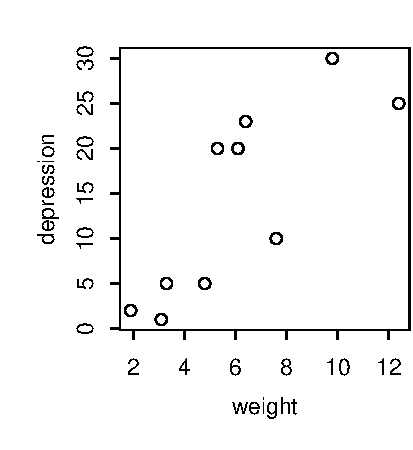
\includegraphics[width=0.45\textwidth]{figs/reg-plt-roller-11_1-1} 

}



\end{knitrout}
  \caption{Plot of \txtt{depression} versus \txtt{weight}, using data
from the data frame \txtt{roller} in the {\em DAAG}
package.}\label{fig:rollerPlot}
\end{figure}

\begin{figure}[H]
\begin{knitrout}
\definecolor{shadecolor}{rgb}{0.969, 0.969, 0.969}\color{fgcolor}\begin{kframe}
\begin{alltt}
\hlkwd{fig11.2}\hlstd{()}
\end{alltt}
\end{kframe}

{\centering 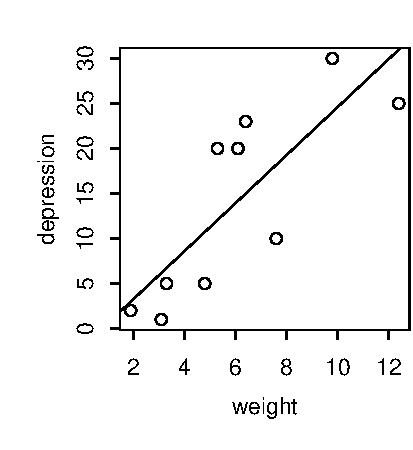
\includegraphics[width=0.45\textwidth]{figs/reg-pltWline-11_2-1} 

}



\end{knitrout}
\caption{This repeats Figure \ref{fig:rollerPlot}, now adding a fitted
  line.}\label{fig:rollerPlot-withline}
\end{figure}

\begin{figure}[H]
\begin{knitrout}
\definecolor{shadecolor}{rgb}{0.969, 0.969, 0.969}\color{fgcolor}\begin{kframe}
\begin{alltt}
\hlkwd{fig11.3}\hlstd{()}
\end{alltt}
\end{kframe}

{\centering 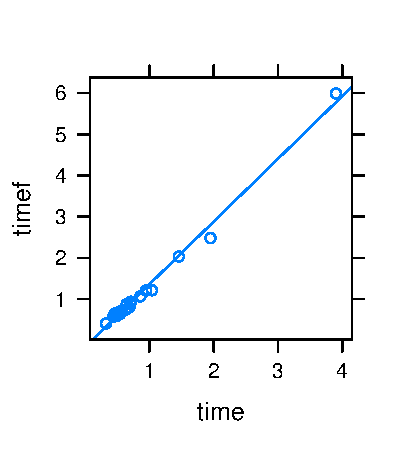
\includegraphics[width=0.45\textwidth]{figs/reg-fVSmTime-11_3-1} 

}



\end{knitrout}
  \caption{Data are for Northern Ireland hill races.
    Record times are compared -- females versus males.  A least squares line
    is added.}\label{fig:nimff}
\end{figure}

\begin{figure}[H]
\begin{knitrout}
\definecolor{shadecolor}{rgb}{0.969, 0.969, 0.969}\color{fgcolor}\begin{kframe}
\begin{alltt}
\hlkwd{fig11.4}\hlstd{()}
\end{alltt}
\end{kframe}

{\centering 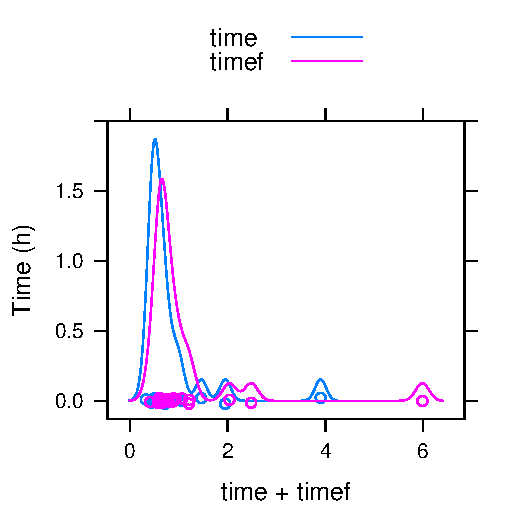
\includegraphics[width=\maxwidth]{figs/reg-mfdensity-11_4-1} 

}



\end{knitrout}
  \caption{Density plot comparison of times between males
    and females.  Note the long tail out to the right,
  already obvious from the diagnostic plots.}\label{fig:skewtime}
\end{figure}

\begin{figure}[H]
\begin{knitrout}
\definecolor{shadecolor}{rgb}{0.969, 0.969, 0.969}\color{fgcolor}\begin{kframe}
\begin{alltt}
\hlkwd{fig11.5A}\hlstd{()}
\hlkwd{fig11.5B}\hlstd{()}
\end{alltt}
\end{kframe}

{\centering 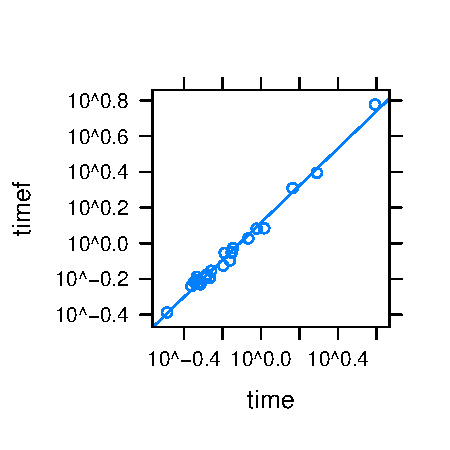
\includegraphics[width=0.47\textwidth]{figs/reg-mVSfTime-11_5-1} 
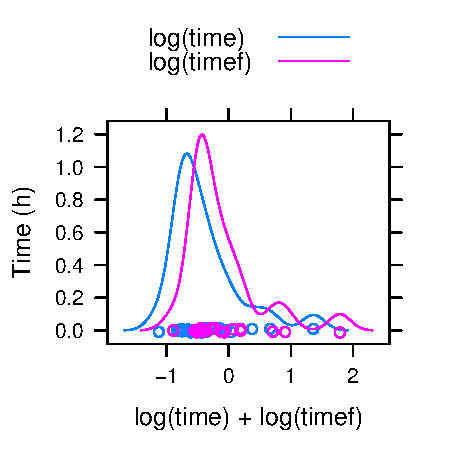
\includegraphics[width=0.47\textwidth]{figs/reg-mVSfTime-11_5-2} 

}



\end{knitrout}
  \caption{In these graphs, female and male times are shown on log scales.
    Panel A shows a density plot comparison. Panel B plots female versus
    male times.
  }\label{fig:skewtime-log}
\end{figure}

\begin{figure}[H]
\begin{knitrout}
\definecolor{shadecolor}{rgb}{0.969, 0.969, 0.969}\color{fgcolor}

{\centering 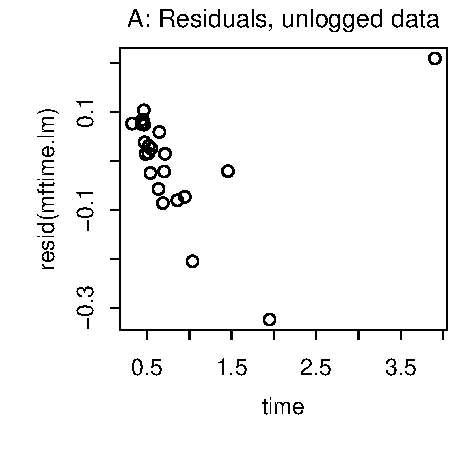
\includegraphics[width=0.47\textwidth]{figs/reg-fig11_6e-1} 
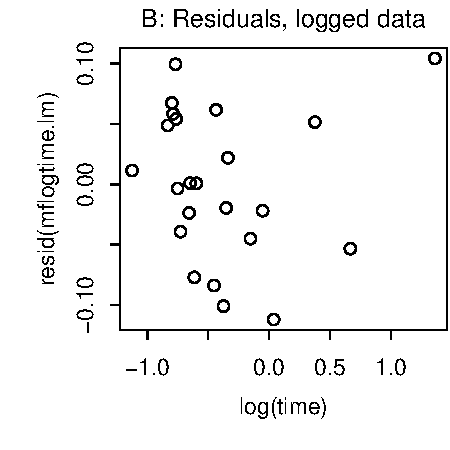
\includegraphics[width=0.47\textwidth]{figs/reg-fig11_6e-2} 

}



\end{knitrout}
\caption{In Panel A, residuals from the line for the unlogged data
  have been plotted against male times.  Panel B repeats the same
  type of plot, now for the regression for the logged data.\label{fig:to-horiz}}
\end{figure}


\begin{figure}[H]
\begin{knitrout}
\definecolor{shadecolor}{rgb}{0.969, 0.969, 0.969}\color{fgcolor}\begin{kframe}
\begin{alltt}
\hlkwd{fig11.7}\hlstd{()}
\end{alltt}
\end{kframe}

{\centering 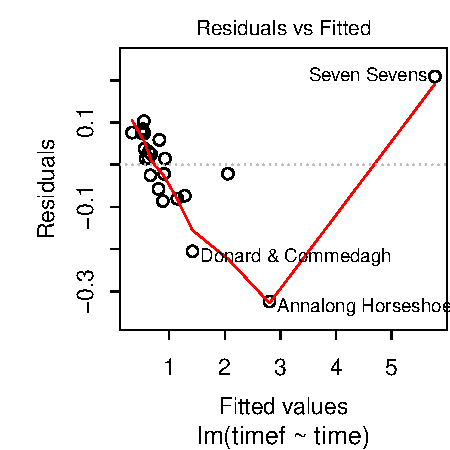
\includegraphics[width=0.23\textwidth]{figs/reg-diag-mf-11_7-1} 
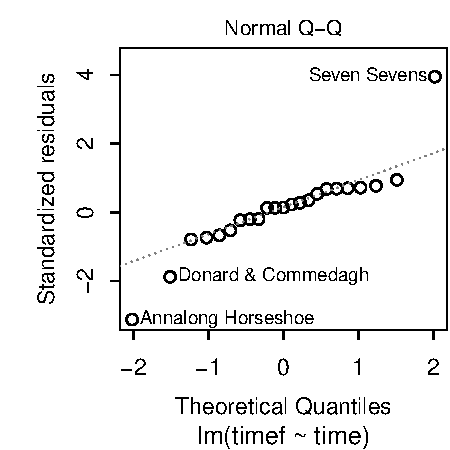
\includegraphics[width=0.23\textwidth]{figs/reg-diag-mf-11_7-2} 
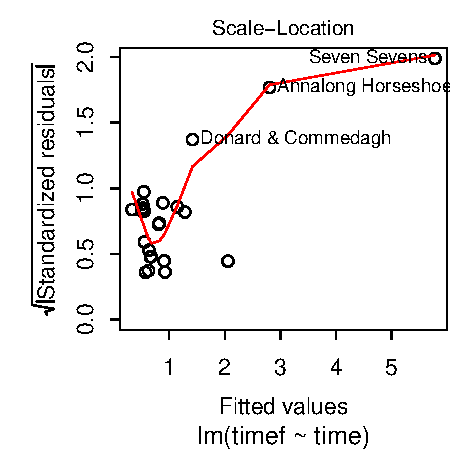
\includegraphics[width=0.23\textwidth]{figs/reg-diag-mf-11_7-3} 
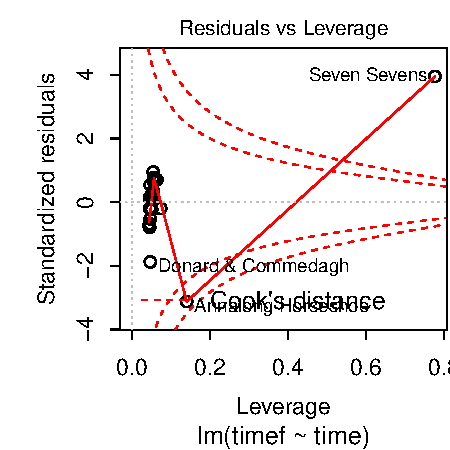
\includegraphics[width=0.23\textwidth]{figs/reg-diag-mf-11_7-4} 

}



\end{knitrout}
\caption{Diagnostic plots from the regession of \txtt{log(timef)} on
  \txtt{log(time)}.}\label{fig:diag-mftime}
\end{figure}

\begin{figure}[H]
\begin{knitrout}
\definecolor{shadecolor}{rgb}{0.969, 0.969, 0.969}\color{fgcolor}\begin{kframe}
\begin{alltt}
\hlkwd{fig11.8}\hlstd{()}
\end{alltt}
\end{kframe}

{\centering 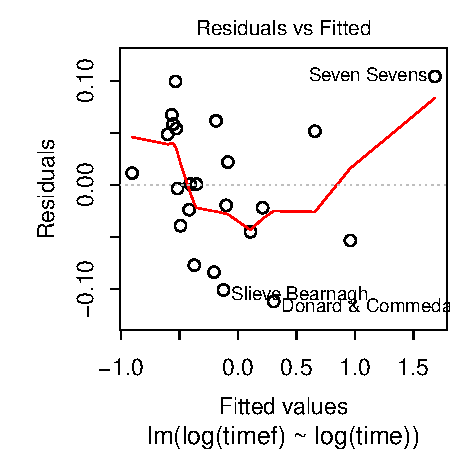
\includegraphics[width=0.23\textwidth]{figs/reg-diag-logmf-11_8-1} 
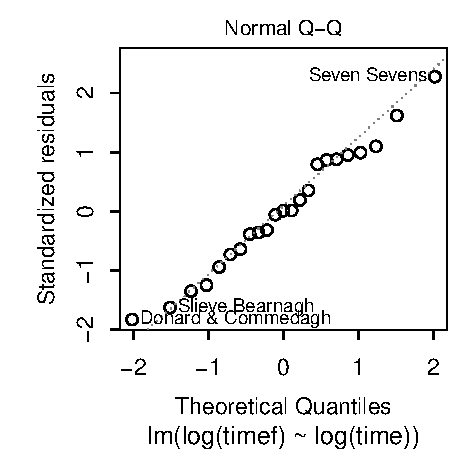
\includegraphics[width=0.23\textwidth]{figs/reg-diag-logmf-11_8-2} 
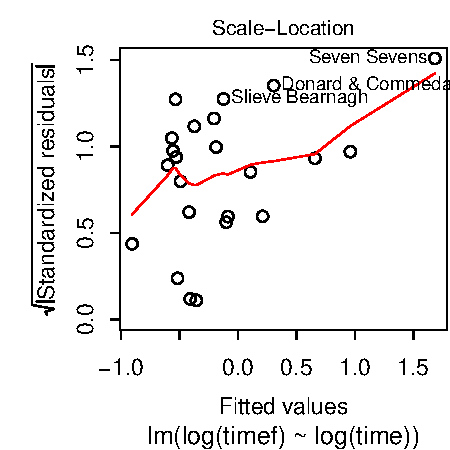
\includegraphics[width=0.23\textwidth]{figs/reg-diag-logmf-11_8-3} 
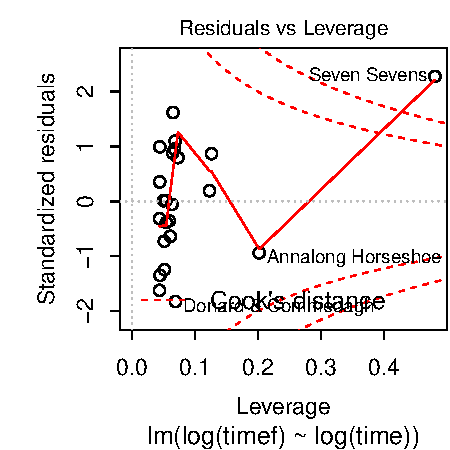
\includegraphics[width=0.23\textwidth]{figs/reg-diag-logmf-11_8-4} 

}



\end{knitrout}
\caption{Diagnostic plots from the regession of \txtt{log(timef)} on
  \txtt{log(time)}.}\label{fig:diag-mftime-log}
\end{figure}

\begin{figure}[H]
\begin{knitrout}
\definecolor{shadecolor}{rgb}{0.969, 0.969, 0.969}\color{fgcolor}\begin{kframe}
\begin{alltt}
\hlkwd{fig11.9}\hlstd{()}
\end{alltt}
\end{kframe}

{\centering 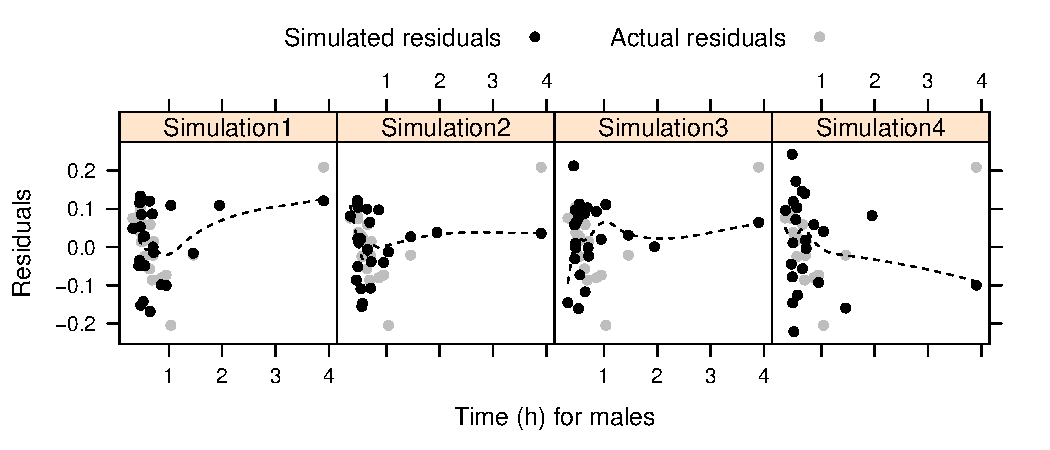
\includegraphics[width=0.97\textwidth]{figs/reg-simscat-11_9-1} 

}



\end{knitrout}
\caption{The plots are four simulations of residuals.  The coefficients
  used, and the standard deviation, are from the fitted least squares
  line.\label{fig:4sim-mftimeres1}}
\end{figure}

\begin{suppfigure}[H]
\begin{knitrout}
\definecolor{shadecolor}{rgb}{0.969, 0.969, 0.969}\color{fgcolor}\begin{kframe}
\begin{alltt}
\hlkwd{suppfig11.1}\hlstd{()}
\end{alltt}
\end{kframe}

{\centering 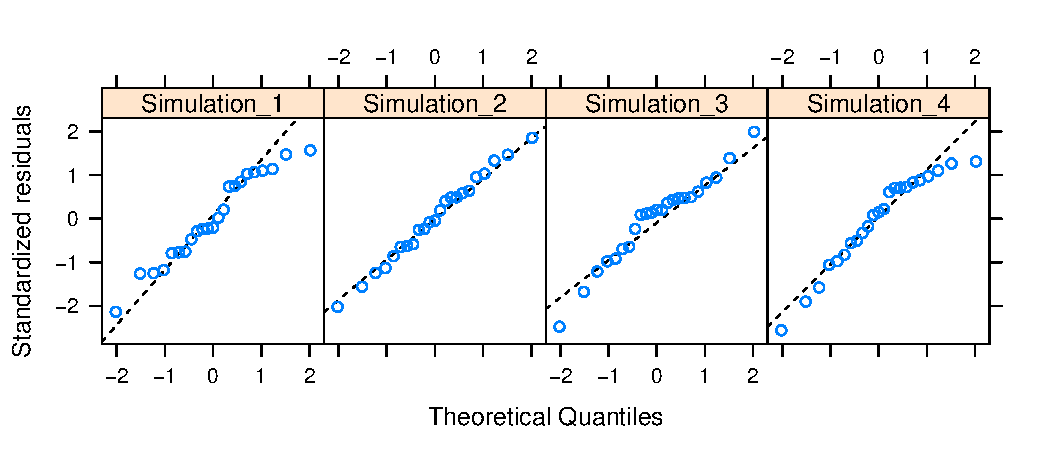
\includegraphics[width=0.97\textwidth]{figs/reg-which2-s11_1e-1} 

}



\end{knitrout}
\caption{Normal probability plots for four sets of simulated
  data.}\label{fig:mftimesimdiag2}
\end{suppfigure}

\begin{suppfigure}[H]
\begin{knitrout}
\definecolor{shadecolor}{rgb}{0.969, 0.969, 0.969}\color{fgcolor}\begin{kframe}
\begin{alltt}
\hlkwd{suppfig11.2}\hlstd{()}
\end{alltt}
\end{kframe}

{\centering 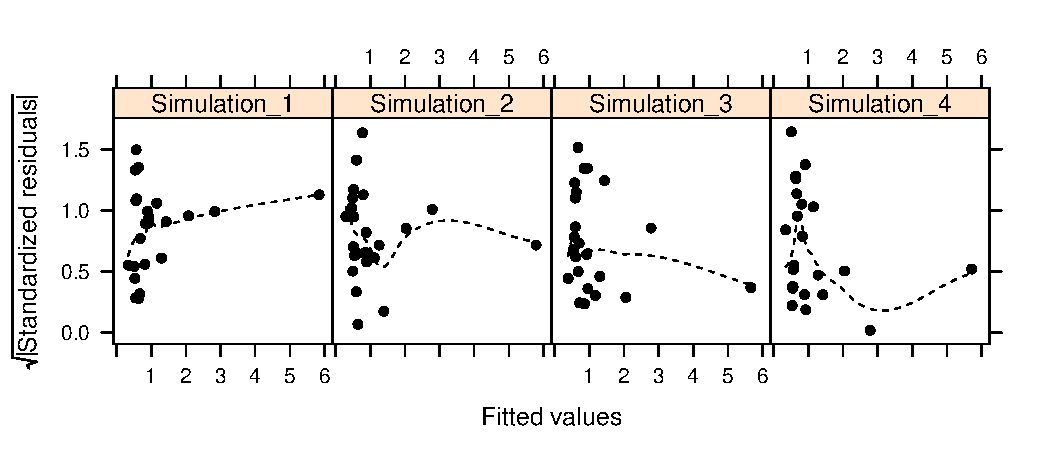
\includegraphics[width=0.97\textwidth]{figs/reg-which3-s11_2e-1} 

}



\end{knitrout}
\caption{These plots, here with simulated data, are designed to
  check for change in variance as the fitted values
  change.\label{fig:mftimecheck3}}
\end{suppfigure}

\begin{suppfigure}[H]
\begin{knitrout}
\definecolor{shadecolor}{rgb}{0.969, 0.969, 0.969}\color{fgcolor}\begin{kframe}
\begin{alltt}
\hlkwd{suppfig11.3}\hlstd{()}
\end{alltt}
\end{kframe}

{\centering 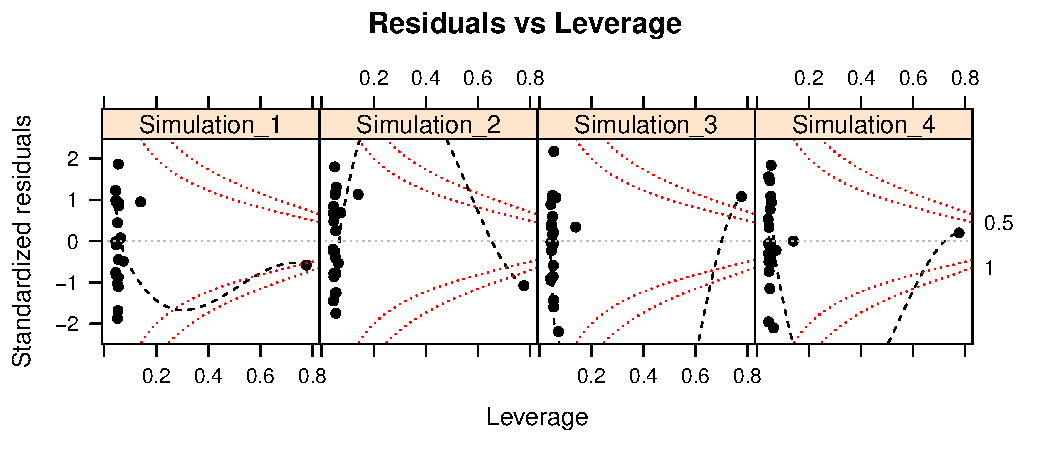
\includegraphics[width=0.97\textwidth]{figs/reg-simdiag3-11_3e-1} 

}



\end{knitrout}
\caption{Scale-location plots for four sets of simulated
  data.}\label{fig:mftimesimdiag3}
\end{suppfigure}

\begin{suppfigure}[H]
\begin{knitrout}
\definecolor{shadecolor}{rgb}{0.969, 0.969, 0.969}\color{fgcolor}\begin{kframe}
\begin{alltt}
\hlkwd{suppfig11.4}\hlstd{()}
\end{alltt}
\end{kframe}

{\centering 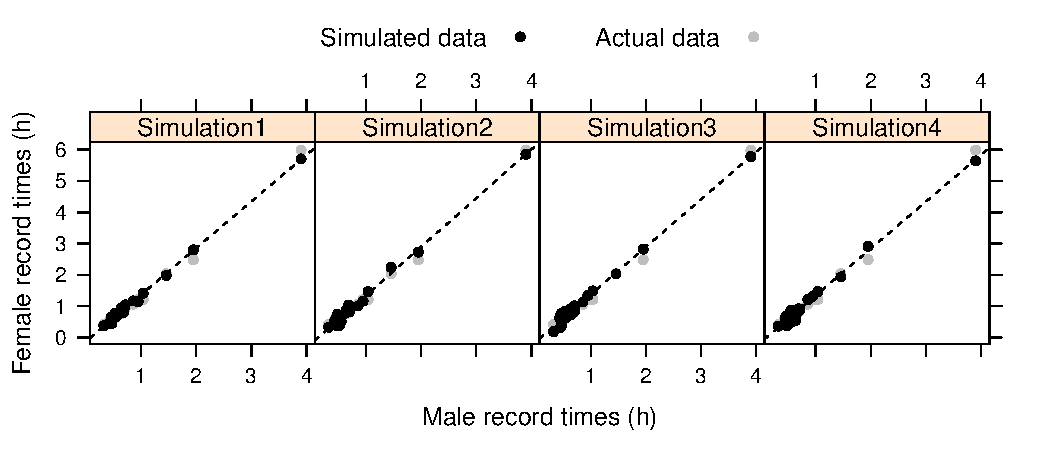
\includegraphics[width=0.97\textwidth]{figs/reg-mftime-sims-s11_4-1} 

}



\end{knitrout}
\vspace*{-9pt}

\caption{The plots are four simulations of points.  The coefficients
  used, and the standard deviation, are from the fitted least squares
  line. The gray points are the data values, which are of course the
same in all 4 plots.}\label{fig:4sim-nimff}
\end{suppfigure}

\begin{figure}[H]
\begin{knitrout}
\definecolor{shadecolor}{rgb}{0.969, 0.969, 0.969}\color{fgcolor}\begin{kframe}
\begin{alltt}
\hlkwd{fig11.10A}\hlstd{()}
\hlkwd{fig11.10B}\hlstd{()}
\end{alltt}
\end{kframe}

{\centering 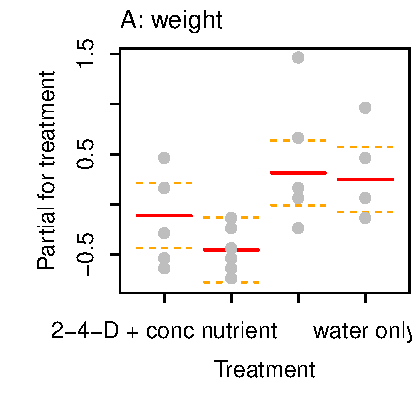
\includegraphics[width=0.47\textwidth]{figs/reg-tomato-11-10e-1} 
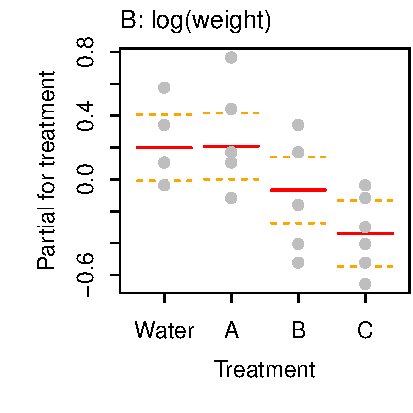
\includegraphics[width=0.47\textwidth]{figs/reg-tomato-11-10e-2} 

}



\end{knitrout}
 \caption{Termplot summary of the one-way analysis of variance result:
(a) for the analysis that uses weights as the outcome variable, and
(b) for the analysis that works with \txtt{log(weight)}}
\label{fig:tomatoterm}
\end{figure}


\begin{figure}[H]
\begin{knitrout}
\definecolor{shadecolor}{rgb}{0.969, 0.969, 0.969}\color{fgcolor}\begin{kframe}
\begin{alltt}
\hlkwd{fig11.11A}\hlstd{()}
\hlkwd{fig11.11B}\hlstd{()}
\end{alltt}
\end{kframe}

{\centering 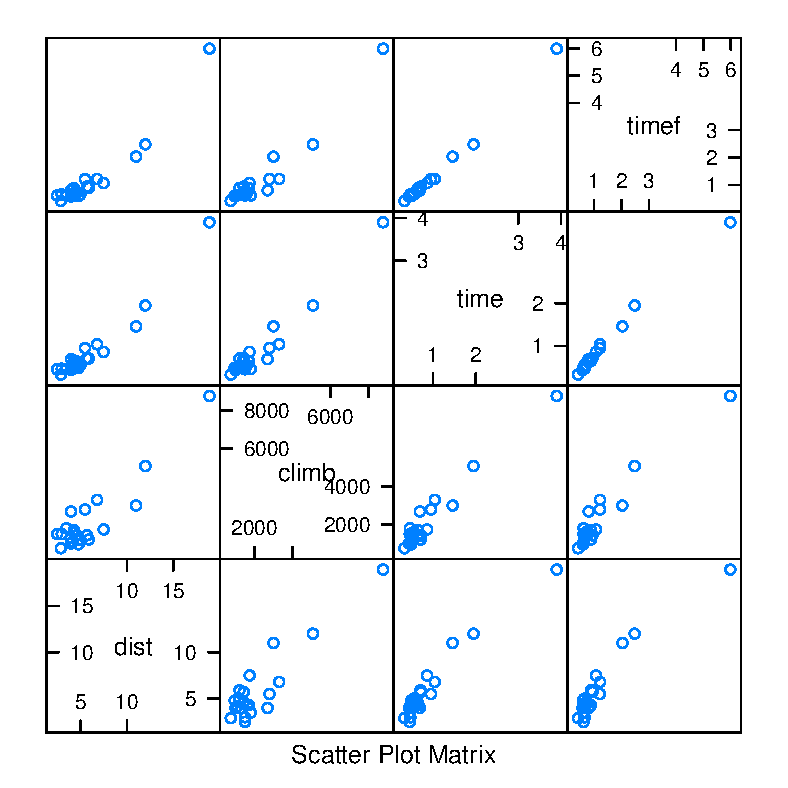
\includegraphics[width=0.48\textwidth]{figs/reg-splot2-ni-11-11e-1} 
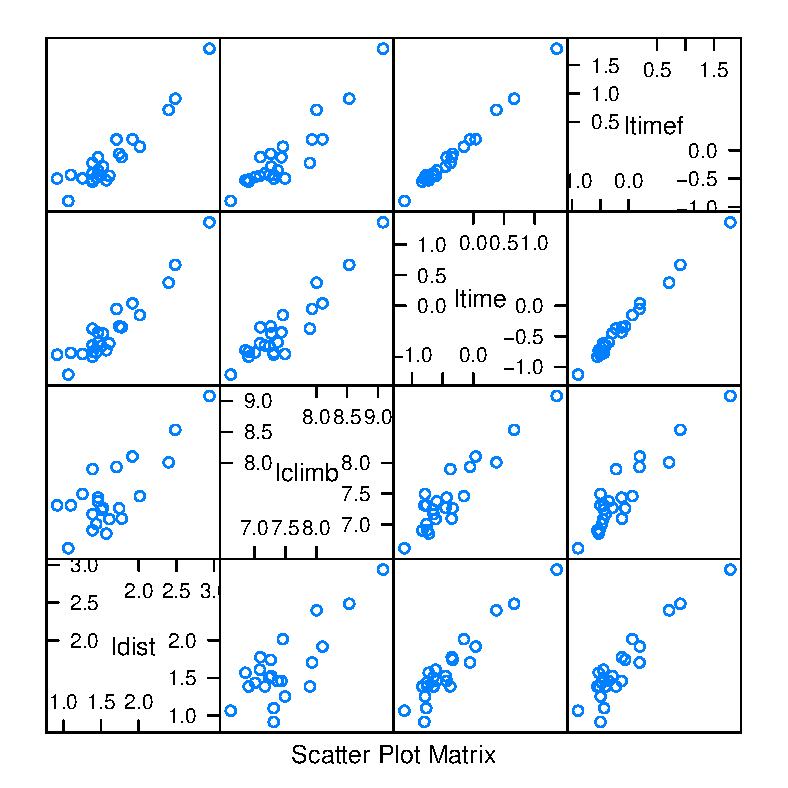
\includegraphics[width=0.48\textwidth]{figs/reg-splot2-ni-11-11e-2} 

}



\end{knitrout}
\caption{Scatterplot matrices for the Northern Ireland mountain racing
  data. In the right panel, code has been added that shows the
  correlations.
\label{fig:nimra-reg}}
\end{figure}



\begin{figure}[H]
\begin{knitrout}
\definecolor{shadecolor}{rgb}{0.969, 0.969, 0.969}\color{fgcolor}\begin{kframe}
\begin{alltt}
\hlkwd{fig11.12}\hlstd{()}
\end{alltt}
\end{kframe}

{\centering 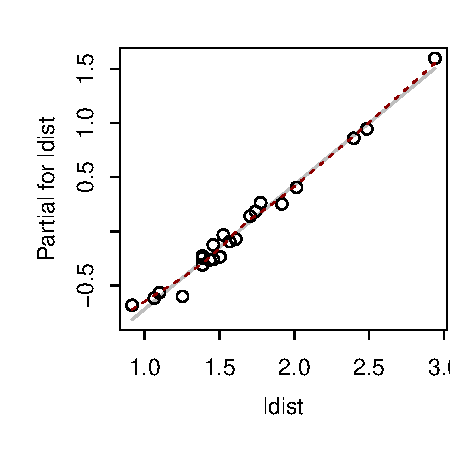
\includegraphics[width=0.48\textwidth]{figs/reg-tplot-ni-11_12-1} 
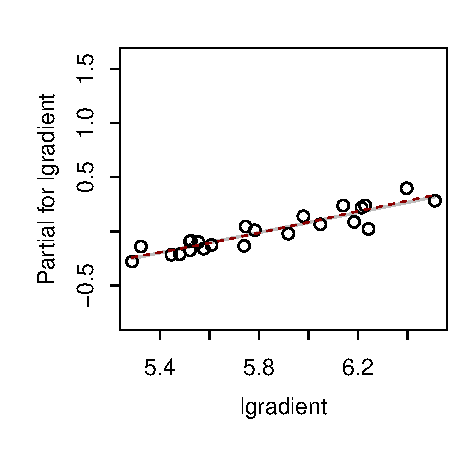
\includegraphics[width=0.48\textwidth]{figs/reg-tplot-ni-11_12-2} 

}



\end{knitrout}
\caption{The vertical scales in both ``term plot'' panels show
  $\log(\rm{time})$, centered to a mean of zero. The partial residuals
  in the left panel are for the effect of $\txtt{ldist}$, while those
  in the right panel are for the effect of $\txtt{lgradient}$, i.e.,
  \txtt{log(climb/dist)}. Smooth curves (dashes) have been passed
  through the points.\label{fig:lnihills-lin}}
\vspace*{-15pt}
\end{figure}

\begin{figure}[H]
\begin{knitrout}
\definecolor{shadecolor}{rgb}{0.969, 0.969, 0.969}\color{fgcolor}\begin{kframe}
\begin{alltt}
\hlkwa{if}\hlstd{(}\hlopt{!}\hlkwd{requireNamespace}\hlstd{(}\hlstr{"quantreg"}\hlstd{,} \hlkwc{quietly}\hlstd{=}\hlnum{TRUE}\hlstd{))}
    \hlkwd{print}\hlstd{(}\hlstr{"As quantreg is not available, trend curve will be omitted."}\hlstd{)}
\hlkwd{fig11.13}\hlstd{()}
\end{alltt}
\end{kframe}

{\centering 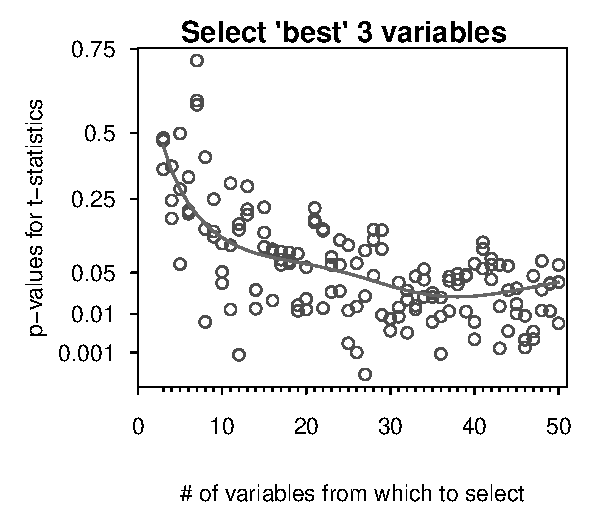
\includegraphics[width=\maxwidth]{figs/reg-bsnVary-11_13-1} 

}



\end{knitrout}
\caption{$p$-values, versus number of variables available for selection,
  when the ``best'' 3 variables were selected by exhaustive search.
  The fitted line estimates the median $p$-value.\label{fig:exhaust}}
\end{figure}

\begin{knitrout}
\definecolor{shadecolor}{rgb}{0.969, 0.969, 0.969}\color{fgcolor}\begin{kframe}
\begin{alltt}
\hlstd{check4Elec} \hlkwb{<-} \hlkwd{exists}\hlstd{(}\hlstr{"Electricity"}\hlstd{)}
\hlkwa{if}\hlstd{(}\hlopt{!}\hlstd{check4Elec)\{}
    \hlkwa{if}\hlstd{(}\hlopt{!}\hlkwd{require}\hlstd{(Ecdat,} \hlkwc{quietly}\hlstd{=}\hlnum{TRUE}\hlstd{))}\hlkwd{stop}\hlstd{(}\hlstr{"Dataset Electricity is not available."}\hlstd{)}
\hlstd{\}}
\hlstd{check4Elec} \hlkwb{<-} \hlnum{TRUE}
\hlkwd{data}\hlstd{(Electricity)}
\end{alltt}
\end{kframe}
\end{knitrout}

\begin{figure}[H]
\parbox[c]{0.7\textwidth}{
\begin{knitrout}
\definecolor{shadecolor}{rgb}{0.969, 0.969, 0.969}\color{fgcolor}\begin{kframe}
\begin{alltt}
\hlkwa{if}\hlstd{(check4Elec)}\hlkwd{fig11.14}\hlstd{()}
\end{alltt}
\end{kframe}

{\centering 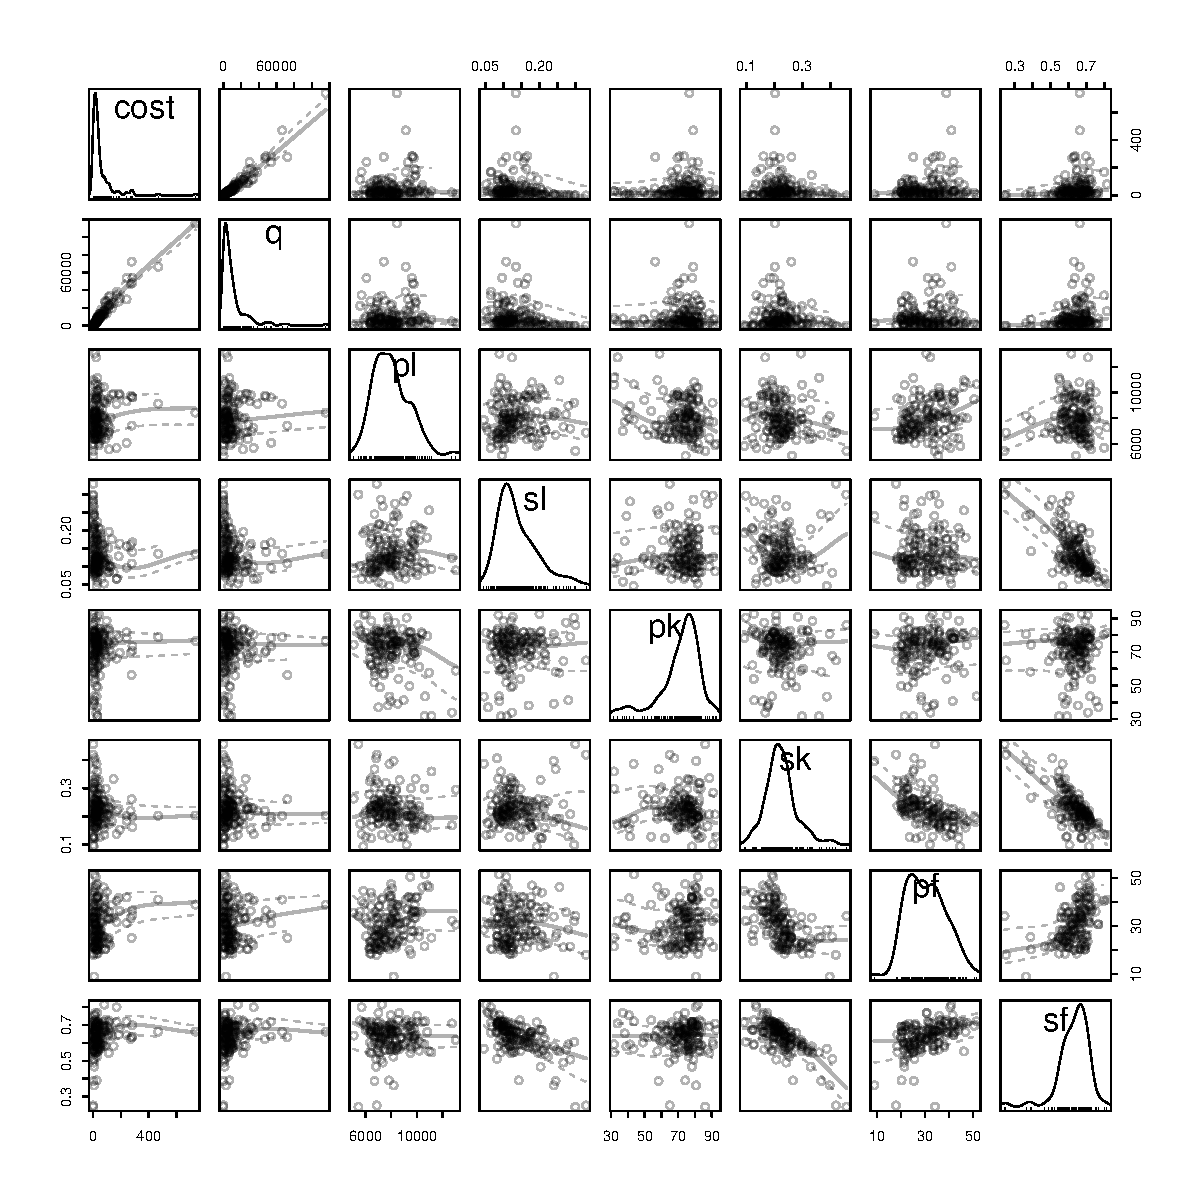
\includegraphics[width=0.775\textwidth]{figs/reg-Elec-spm-11_14-1} 

}



\end{knitrout}
}
\hspace*{0.05\textwidth}
\parbox[c]{0.18\linewidth}{
\small
\begin{list}{}{\leftmargin=2em \setlength{\itemsep}{5pt} \setlength{\parsep}{1pt}}
\setlength{\labelwidth}{3em}
\item[\texttt{cost:}]
 total cost
\item[\texttt{q:}]
 total output
\item[\texttt{pl:}]
 wage rate
\item[\texttt{sl:}]
 cost share, labor
\item[\texttt{pk:}]
 capital price index
\item[\texttt{sk:}]
 cost share,
 capital
\item[\texttt{pf:}]
 fuel price
\item[\texttt{sf:}]
 cost share, fuel
\end{list}
}
\vspace*{-9pt}

\caption{Scatterplot matrix, for the variables in the data set
  \texttt{Electricity}, in the {\em Ecdat} package. Density
  plots are shown in the diagonal.\label{fig:elec-spm}}
\end{figure}

\begin{figure}[H]
\begin{knitrout}
\definecolor{shadecolor}{rgb}{0.969, 0.969, 0.969}\color{fgcolor}\begin{kframe}
\begin{alltt}
\hlkwa{if}\hlstd{(check4Elec)}\hlkwd{fig11.15}\hlstd{()}
\end{alltt}
\end{kframe}

{\centering 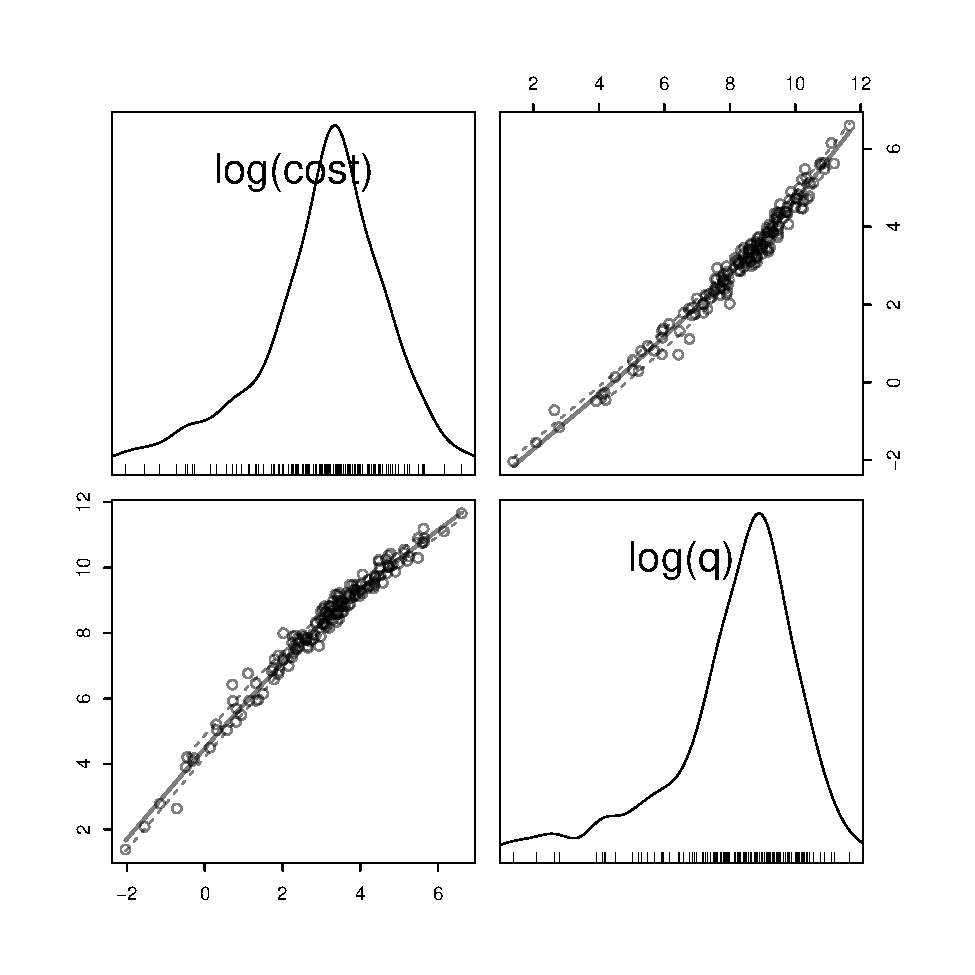
\includegraphics[width=0.45\textwidth]{figs/reg-spm-cost-q-11_15-1} 

}



\end{knitrout}
  \caption{Scatterplot matrix for the logarithms of the variables
    \txtt{cost} and \txtt{q}. Density plots are shown in the
    diagonal.\label{fig:elec-dens}}
\end{figure}



\begin{figure}[H]
\begin{knitrout}
\definecolor{shadecolor}{rgb}{0.969, 0.969, 0.969}\color{fgcolor}\begin{kframe}
\begin{alltt}
\hlkwa{if}\hlstd{(check4Elec)}\hlkwd{fig11.16}\hlstd{()}
\end{alltt}
\end{kframe}

{\centering 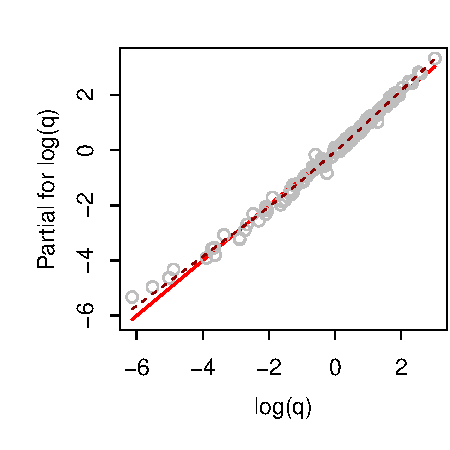
\includegraphics[width=0.24\textwidth]{figs/reg-elec-me-tplot-11_16-1} 
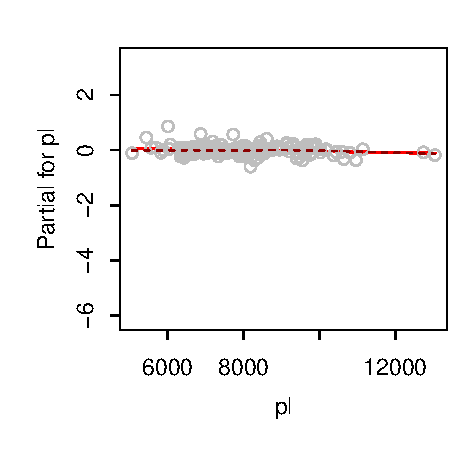
\includegraphics[width=0.24\textwidth]{figs/reg-elec-me-tplot-11_16-2} 
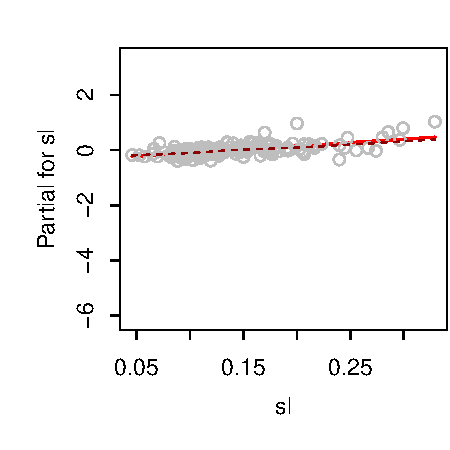
\includegraphics[width=0.24\textwidth]{figs/reg-elec-me-tplot-11_16-3} 
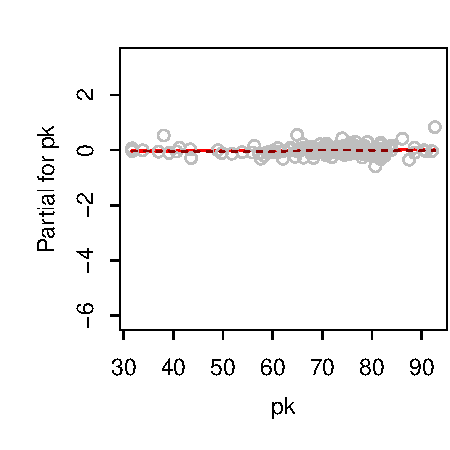
\includegraphics[width=0.24\textwidth]{figs/reg-elec-me-tplot-11_16-4} 
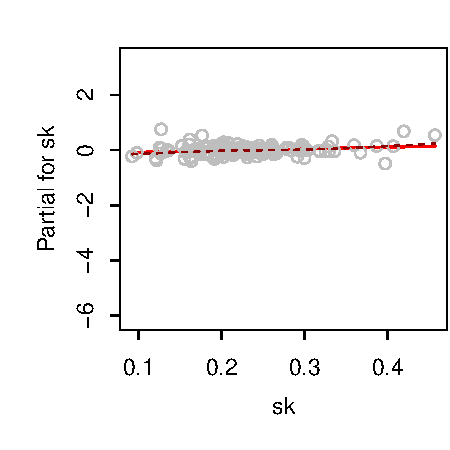
\includegraphics[width=0.24\textwidth]{figs/reg-elec-me-tplot-11_16-5} 
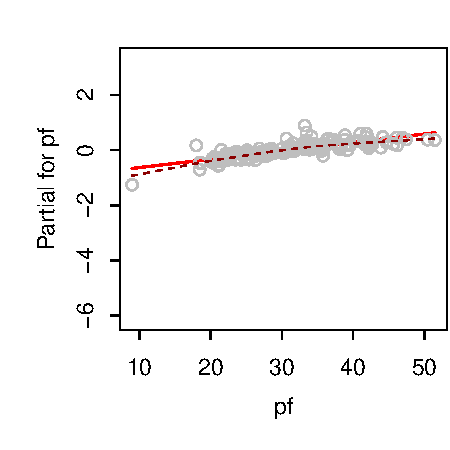
\includegraphics[width=0.24\textwidth]{figs/reg-elec-me-tplot-11_16-6} 
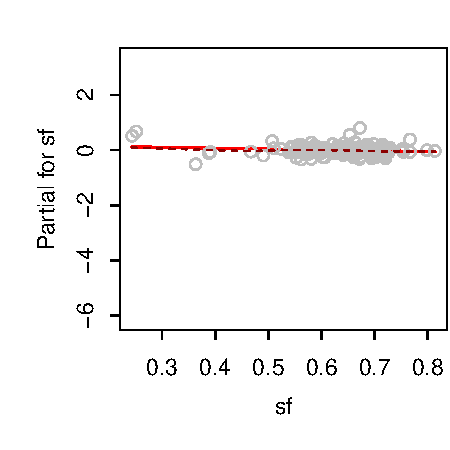
\includegraphics[width=0.24\textwidth]{figs/reg-elec-me-tplot-11_16-7} 

}



\end{knitrout}
\caption{Termplot summary for the model that has been fitted to the
  \texttt{Electricity} dataset.\label{fig:elec-log-tplot}}
\end{figure}



\begin{figure}[H]
\begin{knitrout}
\definecolor{shadecolor}{rgb}{0.969, 0.969, 0.969}\color{fgcolor}\begin{kframe}
\begin{alltt}
\hlstd{opar} \hlkwb{<-} \hlkwd{par}\hlstd{(}\hlkwc{mar}\hlstd{=}\hlkwd{c}\hlstd{(}\hlnum{4}\hlstd{,}\hlnum{4}\hlstd{,}\hlnum{2.5}\hlstd{,}\hlnum{0.6}\hlstd{))}

\hlkwd{fig11.17A}\hlstd{()}
\hlkwd{fig11.17B}\hlstd{()}
\hlkwd{par}\hlstd{(opar)}
\end{alltt}
\end{kframe}

{\centering 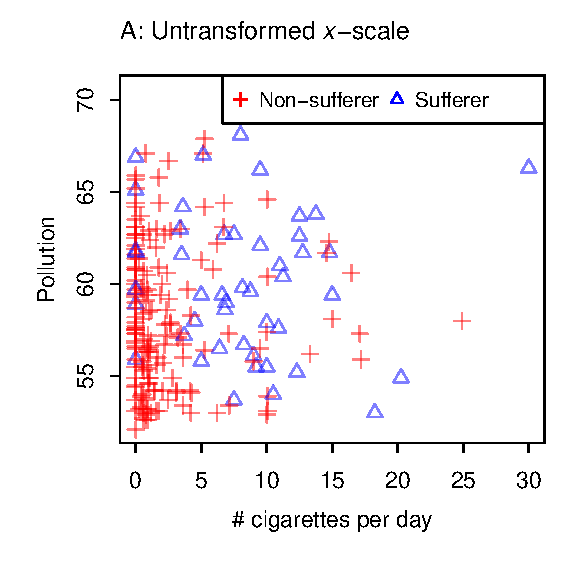
\includegraphics[width=0.47\textwidth]{figs/reg-bronchitAB-1} 
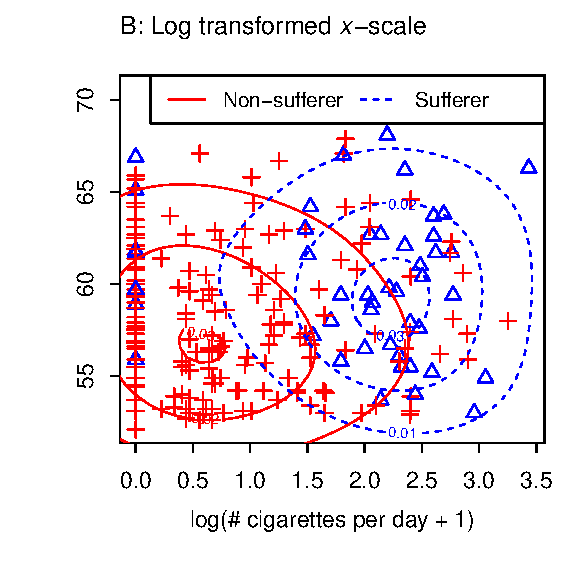
\includegraphics[width=0.47\textwidth]{figs/reg-bronchitAB-2} 

}



\end{knitrout}
\caption{Panel A plots \txtt{poll} (pollution level) against
  \txtt{cig} (number of cigarettes per day).  In panel B, the
  $x$-scale shows the logarithm of the number of cigarettes per
  day.\label{fig:cig-poll}}
\end{figure}



\begin{figure}[H]
\begin{knitrout}
\definecolor{shadecolor}{rgb}{0.969, 0.969, 0.969}\color{fgcolor}\begin{kframe}
\begin{alltt}
\hlkwd{fig11.18}\hlstd{()}
\end{alltt}
\end{kframe}

{\centering 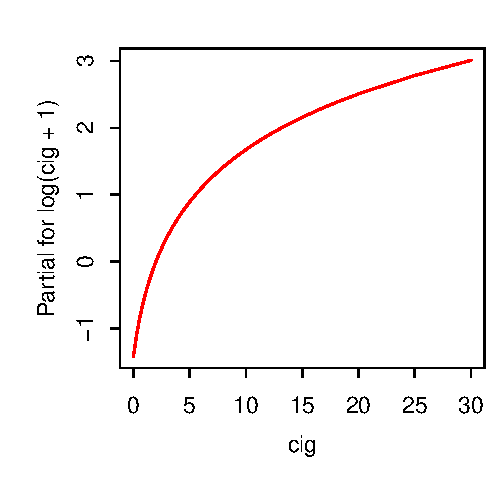
\includegraphics[width=0.47\textwidth]{figs/reg-cig2-tplot-11_18-1} 
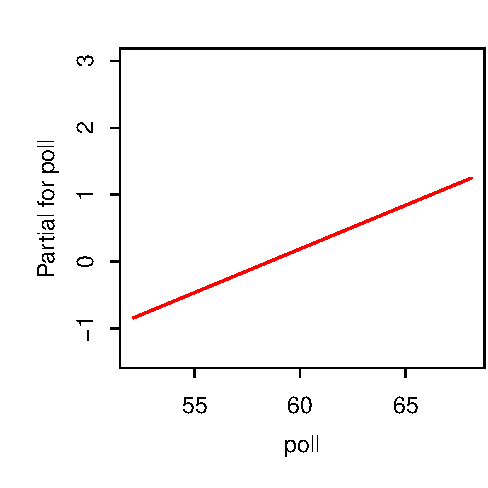
\includegraphics[width=0.47\textwidth]{figs/reg-cig2-tplot-11_18-2} 

}



\end{knitrout}
\caption{The panels show the contributions that the respective terms
  make to the fitted values (logit of probability of bronchitis), when
  the other term is held constant.\label{fig:xy-cig}}
\end{figure}

\end{document}


